\chapter{Continuity of Functions}

\section{Limit of a function.}
Let $X$ and $Y$ be two metric spaces equipped with some distance metrics $d_X, d_Y$.
Let $E\subset Y$ and $f:E\to Y$, then we denote the \textit{limit of the function $f$} as it approaches the point $p\in X$ as $\lim_{x\to p}f(x)$ and define it as:
$f(x)\to q$ as $x\to p\equiv \lim_{x\to p} f(x)=q,$ if for any $\varepsilon>0\,\exists \delta_\varepsilon>0$ such that $d_Y(f(x),q) < \varepsilon$ if $0<d_X(x,p)<\delta_\varepsilon, x\in E$.
Note that speaking of the limit of a function at an isolated point (i.e., if $p\in E$ but $p\notin E'$) is irrelevant.
\begin{figure}[!ht]
    \centering
    \scalebox{.80}{% Pattern Info
 
\tikzset{
pattern size/.store in=\mcSize, 
pattern size = 5pt,
pattern thickness/.store in=\mcThickness, 
pattern thickness = 0.3pt,
pattern radius/.store in=\mcRadius, 
pattern radius = 1pt}
\makeatletter
\pgfutil@ifundefined{pgf@pattern@name@_bt4epe2mx}{
\pgfdeclarepatternformonly[\mcThickness,\mcSize]{_bt4epe2mx}
{\pgfqpoint{0pt}{0pt}}
{\pgfpoint{\mcSize+\mcThickness}{\mcSize+\mcThickness}}
{\pgfpoint{\mcSize}{\mcSize}}
{
\pgfsetcolor{\tikz@pattern@color}
\pgfsetlinewidth{\mcThickness}
\pgfpathmoveto{\pgfqpoint{0pt}{0pt}}
\pgfpathlineto{\pgfpoint{\mcSize+\mcThickness}{\mcSize+\mcThickness}}
\pgfusepath{stroke}
}}
\makeatother
\tikzset{every picture/.style={line width=0.75pt}} %set default line width to 0.75pt        

\begin{tikzpicture}[x=0.75pt,y=0.75pt,yscale=-1,xscale=1]
%uncomment if require: \path (0,300); %set diagram left start at 0, and has height of 300

%Shape: Polygon Curved [id:ds7313279635399221] 
\draw   (96,85) .. controls (97,64) and (230,52) .. (230,70) .. controls (230,88) and (194,71) .. (214,101) .. controls (234,131) and (175,149) .. (155,119) .. controls (135,89) and (95,106) .. (96,85) -- cycle ;
%Shape: Ellipse [id:dp9151376985030744] 
\draw  [pattern=_bt4epe2mx,pattern size=6pt,pattern thickness=0.75pt,pattern radius=0pt, pattern color={rgb, 255:red, 128; green, 128; blue, 128}] (142.28,81.2) .. controls (146.96,71.19) and (164.94,69.7) .. (182.46,77.88) .. controls (199.97,86.05) and (210.39,100.79) .. (205.72,110.8) .. controls (201.04,120.81) and (183.06,122.3) .. (165.54,114.12) .. controls (148.03,105.95) and (137.61,91.21) .. (142.28,81.2) -- cycle ;
%Shape: Polygon Curved [id:ds132327224769744] 
\draw   (281,58) .. controls (301,48) and (289,25) .. (340,32) .. controls (391,39) and (351,88) .. (371,118) .. controls (391,148) and (334,146) .. (314,116) .. controls (294,86) and (261,68) .. (281,58) -- cycle ;
%Curve Lines [id:da8275404505595068] 
\draw [color={rgb, 255:red, 0; green, 0; blue, 0 }  ,draw opacity=1 ] [dash pattern={on 0.84pt off 2.51pt}]  (201,117) .. controls (259.12,92.37) and (303.65,137.61) .. (346.54,139.92) ;
\draw [shift={(348.5,140)}, rotate = 181.32] [color={rgb, 255:red, 0; green, 0; blue, 0 }  ,draw opacity=1 ][line width=0.75]    (10.93,-3.29) .. controls (6.95,-1.4) and (3.31,-0.3) .. (0,0) .. controls (3.31,0.3) and (6.95,1.4) .. (10.93,3.29)   ;

%Curve Lines [id:da9060207894942087] 
\draw [color={rgb, 255:red, 0; green, 0; blue, 0 }  ,draw opacity=1 ] [dash pattern={on 0.84pt off 2.51pt}]  (148,75) .. controls (206.71,50.12) and (249.57,27.23) .. (316,30.94) ;
\draw [shift={(317,31)}, rotate = 183.42] [color={rgb, 255:red, 0; green, 0; blue, 0 }  ,draw opacity=1 ][line width=0.75]    (10.93,-3.29) .. controls (6.95,-1.4) and (3.31,-0.3) .. (0,0) .. controls (3.31,0.3) and (6.95,1.4) .. (10.93,3.29)   ;

%Shape: Circle [id:dp3248341251389637] 
\draw   (143.8,87.78) .. controls (143.66,80.75) and (149.24,75.06) .. (156.27,75.06) .. controls (163.29,75.06) and (169.1,80.75) .. (169.24,87.78) .. controls (169.39,94.8) and (163.8,100.5) .. (156.78,100.5) .. controls (149.75,100.5) and (143.94,94.8) .. (143.8,87.78) -- cycle ;
%Shape: Circle [id:dp6767491936815082] 
\draw   (297.92,67.28) .. controls (297.72,56.94) and (305.93,48.56) .. (316.27,48.56) .. controls (326.61,48.56) and (335.16,56.94) .. (335.37,67.28) .. controls (335.57,77.62) and (327.36,86) .. (317.02,86) .. controls (306.68,86) and (298.13,77.62) .. (297.92,67.28) -- cycle ;
%Curve Lines [id:da5288665296815309] 
\draw [color={rgb, 255:red, 0; green, 0; blue, 0 }  ,draw opacity=1 ]   (168,95) .. controls (227,70) and (244.5,81.5) .. (311.5,85.5) ;


%Curve Lines [id:da027014413608954735] 
\draw [color={rgb, 255:red, 0; green, 0; blue, 0 }  ,draw opacity=1 ]   (151.5,75.5) .. controls (210.5,50.5) and (249.27,44.56) .. (316.27,48.56) ;



% Text Node
\draw (131,84) node   {$E$};
% Text Node
\draw (143,135) node   {$X$};
% Text Node
\draw (392.5,132.5) node   {$Y$};
% Text Node
\draw (157.5,83.5) node   {$p$};
% Text Node
\draw (184,106) node   {$\mathcal{N}_{{\delta }_{\varepsilon }}( p)$};
% Text Node
\draw (318.5,63) node   {$q$};
% Text Node
\draw (332.5,91.5) node   {$\mathcal{N}_{\varepsilon }( q)$};
% Text Node
\draw (253,119) node   {$f:E\rightarrow X$};


\end{tikzpicture}}
    \caption{Pictorial mapping of neighbourhood of $p\in E$ to $q\in Y$ under $f$}
    \label{fig:contNeigh}
\end{figure}

This definition is represented in Fig. \ref{fig:contNeigh} where $\mathcal{N}_{\delta_\varepsilon}(p)$ gets mapped to $\mathcal{N}_\varepsilon (q)$.
Since $\varepsilon$ is arbitrary, the neighbourhood around point $q$ can be made arbitrarily small, and still one would be able to find a corresponding point $x$ in the $\delta_\varepsilon$ neighbourhood of $p$.
Note that there could be a hole in the neighbourhood $\mathcal{N}_{\varepsilon}$ at $f(p)$.
That is, for the definition of the limit $\lim_{x\to p} f(x)$, the value of the function at $p$ is irrelevant.

An alternate \textit{sequential definition} of the limit of a function at a point uses the preservation of sequential limits under functional mappings.
For any sequence $p_n$ in $E$, if $p_n\to p, p_n\neq p$ holds then $f(p_n)\to q$ $\iff \lim_{x\to p}f(x)=q$.
Note that similar definitions of limit hold for functions in higher dimensions.
That is, $\lim_{x\to p}f(x)=q=(q_1,\cdots,q_k) \iff \lim_{x\to p}f_i(x)=q_i$ for $i=1,2,\cdots,k$.

The sequential definition of limits of a function is very useful since it helps us to borrow the important results of sequence convergence algebra, and use them to automatically get limit algebra results.
These limit algebra results are as follows.
If $\lim_{x\to p}f(x)$, $\lim_{x\to p}g(x)$ exist, then
\begin{enumerate}[label=(\roman*)]
    \item  $\lim_{x\to p}\alpha f(x) + \beta g(x) = \alpha \lim_{x\to p}f(x) + \beta \lim_{x\to p} g(x)$
    \item $\lim_{x\to p} f(x)\cdot g(x) = \lim_{x\to p}f(x)\cdot \lim_{x\to p}g(x)$
    \item $\lim_{x\to p} \dfrac{f(x)}{g(x)} = \dfrac{\lim_{x\to p}f(x)}{\lim_{x\to p}g(x)}$\\
    provided $\lim_{x\to p}g(x)\neq 0$ and $g(x)\neq 0$.
\end{enumerate}

\subsection{Limits at infinity.}
Recall that $\bar{\reals}=\reals\cup\{-\infty,+\infty\}$. We can define neighbourhoods in $\bar{\reals}$ as $(x-r,x+r)$ if $x\in\reals, (a,+\infty)$ when $x=+\infty$, and $(-\infty,b)$ when $x=-\infty$ ($a,b\in\reals$).
If $E\subset\reals$, then $+\infty$ is a limit point of $E$ iff $E$ is unbounded above, and $-\infty$ is a limit point if $E$ iff $E$ is unbounded below.
Now if $+\infty\in E',f:E\to\reals,$ we can talk about $\lim_{x\to\infty}f(x)=L\in\reals\iff \abs{f(x)-L}<\varepsilon$ if $x>a_\varepsilon,x\in E,\lim_{x\to a}f(x)=+\infty$ if $a\in E'$.

However, one has to be aware of indeterminate forms such as $\infty-\infty,0\cdot(\pm\infty),\pm\infty/\pm\infty$ when applying algebraic properties to limits.

\section{Continuity of a function.}
Using the definition of limits of a function, we can now define what it means for a function to be continuous at a point.
A function $f:E\to Y$ is continuous at a point $p$ if for any $\varepsilon>0$, $\exists \delta\varepsilon >0$ such that $d_Y(f(x),f(p))< \varepsilon$ if $d_X(x,p)<\delta_\varepsilon$ and $x\in E$.
Or, $f\left(\mathcal{N}_{\delta_\varepsilon}(p)\cap E\right) \subset \mathcal{N}_\varepsilon(f(p))$.
Comparing this with the definition of a limit, we find one key difference.
For the definition of a limit, the point $p\in E'$ is a limit point.

This has two consequences.
For some $f:E\to Y$ and $p\in E$
\begin{enumerate}
\item If $p\in E'$ then if $f$ is continuous at $p \iff \lim{x\to p} f(x) = f(p)$
\item If $p\notin E'$, or $p$ is an isolated point, then \textbf{any} function is continuous at $p$
\end{enumerate}

\subsection{Continuity of Compositions.}
Suppose $a\in A\subset X, b\in B\subset Y$.
Further suppose $f:A\to Y, f(A)\subset B$ and $g:B\to Z$.
If we define $g\circ f (x)=g(f(x)), x\in A$, then $g\circ f:A\to Z$, then the continuity of $f$ at $a$ and $g$ at $f(x)$ implies the continuity of $g\circ f$ at $a$.
This is a consequence of the sequential characterization of continuity.

\subsection{Global Continuity Theorem.}
Global continuity theorem states that for continuous functions, the pre-image of any open (closed) set is open (closed) [see Fig. \ref{fig:gct}].
\begin{theorem}[Global Continuity Theorem.]
A function $f:E\to Y$ is continuous $\iff$ for \emph{any} open set $V\subset Y, f^{-1}(V)$ is also open.
\end{theorem}
As a consequence, the pre-image of a closed set is also closed under continuous functions since if $V (f^{-1}(V))$  is open, $V^c (f^{-1}(V^c) = f^{-1}(V^c)^c)$ is closed.
\begin{figure}[!ht]
    \centering
    \scalebox{0.80}{


\tikzset{every picture/.style={line width=0.75pt}} %set default line width to 0.75pt        

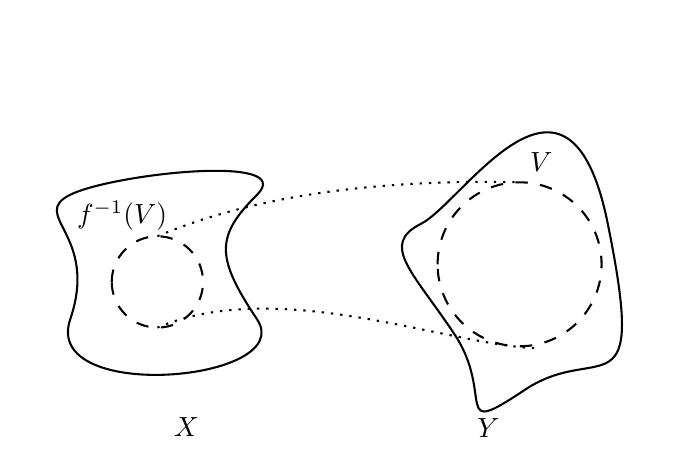
\begin{tikzpicture}[x=0.75pt,y=0.75pt,yscale=-1,xscale=1]
%uncomment if require: \path (0,488); %set diagram left start at 0, and has height of 488

%Shape: Polygon Curved [id:ds026328184733499738] 
\draw   (94,238) .. controls (114,228) and (204,218) .. (184,238) .. controls (164,258) and (164,268) .. (184,298) .. controls (204,328) and (80,339) .. (94,298) .. controls (108,257) and (74,248) .. (94,238) -- cycle ;
%Shape: Polygon Curved [id:ds5677540075211358] 
\draw   (263,252) .. controls (283,242) and (334,158) .. (353,252) .. controls (372,346) and (349,308) .. (313,332) .. controls (277,356) and (299,335) .. (279,305) .. controls (259,275) and (243,262) .. (263,252) -- cycle ;
%Shape: Circle [id:dp6087537463141861] 
\draw  [dash pattern={on 4.5pt off 4.5pt}] (114,280) .. controls (114,267.85) and (123.85,258) .. (136,258) .. controls (148.15,258) and (158,267.85) .. (158,280) .. controls (158,292.15) and (148.15,302) .. (136,302) .. controls (123.85,302) and (114,292.15) .. (114,280) -- cycle ;
%Shape: Circle [id:dp5294184080370192] 
\draw  [dash pattern={on 4.5pt off 4.5pt}] (271,271.5) .. controls (271,249.68) and (288.68,232) .. (310.5,232) .. controls (332.32,232) and (350,249.68) .. (350,271.5) .. controls (350,293.32) and (332.32,311) .. (310.5,311) .. controls (288.68,311) and (271,293.32) .. (271,271.5) -- cycle ;
%Curve Lines [id:da8515105365836626] 
\draw [color={rgb, 255:red, 0; green, 0; blue, 0 }  ,draw opacity=1 ] [dash pattern={on 0.84pt off 2.51pt}]  (136,258) .. controls (195,233) and (267,231) .. (310.5,232) ;


%Curve Lines [id:da8016838777386179] 
\draw [color={rgb, 255:red, 0; green, 0; blue, 0 }  ,draw opacity=1 ] [dash pattern={on 0.84pt off 2.51pt}]  (136,302) .. controls (195,277) and (276.5,311) .. (320,312) ;



% Text Node
\draw (150,350) node   {$X$};
% Text Node
\draw (295.5,350.5) node   {$Y$};
% Text Node
\draw (321,222) node   {$V$};
% Text Node
\draw (119,248) node   {$f^{-1}( V)$};


\end{tikzpicture}}
    \caption{Pre-image of an open set under a continuous function}
    \label{fig:gct}
\end{figure}

\section{Compactness and Continuity.}
Compactness is preserved by continuous functions.
That is, if $X$ is  compact metric space and $f:X\to Y$ is continuous, then $f(X)$ is also compact.
This is a consequence of global continuity theorem applied to the definition of compactness (finite open sub-cover for any cover of the set $f(X)$).

\subsection{Continuity of inverse.}
If $X$ is compact and $f:X\to Y$ continuous and invertible, then its inverse $f^{-1}:Y\to X$ is also continuous.

The continuity of inverse functions can fail for non-compact sets.
For example, $f:[0,2\pi)\to\reals^2$ be defines as $f(t) = (\cos{t},\sin{t})$.
The continuity of this function breaks at $(1,0)\in\reals^2$.
$f^{-1}(1,0)=0$, and $\left(\cos{1/n},-\sin{1/n}\right)\to (1,0)$ as $n\to\infty$, but, $f^{-1}\left(\cos{\frac{1}{n}},-\sin{\frac{1}{n}}\right)= 2\pi-\frac{1}{n}=2\pi$. 

\subsection{Euclidean spaces and continuity.}
If $X$ is compact and $f:X\to \reals^k$, then $f$ is bounded.
That is, $\exists M>0$ such that $\abs{f(x)}\leq M\,\forall x\in X$.
\begin{remark}
A special case arises when $f$ maps to $reals$, i.e., $f:X\to \reals$.
If $f$ is continuous and $X$ compact, then $\sup$ and $\inf$ of $f$ are attained in $X$.
That is, $\exists x^*,x_*\in X$ such that $f(x_*)=\inf_{x\in X}f(x)=m$ and $f(x^*)=\sup_{x\in X}f(x)=M$. 
\end{remark}

\section{Uniform Continuity.}
Uniform continuity is a stronger notion which says that the neighbourhood of radius $\delta_\varepsilon$ around a point $x$ gets mapped to a neighbourhood of radius $\varepsilon$.
Further, there exists $\delta_\varepsilon$ such that the \emph{same} $\delta_\varepsilon$ works for all points $x\in X$.

That is, for any $\varepsilon>0,\,\exists \delta_\varepsilon>0$ such that $d_Y(f(p),f(x))<\varepsilon$ if $d_X(p,x)<\delta_\varepsilon$ for \emph{any} $x\in X$.
\begin{theorem}
If $X$ is compact, $f:X\to Y$ continuous $\implies f:X\to Y$ is uniformly continuous.
\end{theorem}

\section{Continuity and Connectedness.}
Continuity preserves connctedness.
Suppose $f:X\to Y$ is continuous  and $E\subset X$ is connected, then $f(E)\subset Y$ is connected as well.

This is not hard to visualize as shown in Fig. \ref{fig:contConnect}.
Suppose the image $f(E)$ of a connected set $E$ is disconnected.
This would result in a contradiction of $f$ being discontinuous since there would be some points for which the pre-image of some $\varepsilon$ neighbourhood does not lie in the connected set $E$.
The only way $f$ would be continuous, is for $E$ to be disconnected too!
This contradicts with the assumption that $E$ is connected.
\begin{figure}[!ht]
    \centering
    \scalebox{0.75}{


% Pattern Info
 
\tikzset{
pattern size/.store in=\mcSize, 
pattern size = 5pt,
pattern thickness/.store in=\mcThickness, 
pattern thickness = 0.3pt,
pattern radius/.store in=\mcRadius, 
pattern radius = 1pt}
\makeatletter
\pgfutil@ifundefined{pgf@pattern@name@_3ey3x60w6}{
\pgfdeclarepatternformonly[\mcThickness,\mcSize]{_3ey3x60w6}
{\pgfqpoint{0pt}{-\mcThickness}}
{\pgfpoint{\mcSize}{\mcSize}}
{\pgfpoint{\mcSize}{\mcSize}}
{
\pgfsetcolor{\tikz@pattern@color}
\pgfsetlinewidth{\mcThickness}
\pgfpathmoveto{\pgfqpoint{0pt}{\mcSize}}
\pgfpathlineto{\pgfpoint{\mcSize+\mcThickness}{-\mcThickness}}
\pgfusepath{stroke}
}}
\makeatother

% Pattern Info
 
\tikzset{
pattern size/.store in=\mcSize, 
pattern size = 5pt,
pattern thickness/.store in=\mcThickness, 
pattern thickness = 0.3pt,
pattern radius/.store in=\mcRadius, 
pattern radius = 1pt}
\makeatletter
\pgfutil@ifundefined{pgf@pattern@name@_qsk0qv6vp}{
\pgfdeclarepatternformonly[\mcThickness,\mcSize]{_qsk0qv6vp}
{\pgfqpoint{0pt}{-\mcThickness}}
{\pgfpoint{\mcSize}{\mcSize}}
{\pgfpoint{\mcSize}{\mcSize}}
{
\pgfsetcolor{\tikz@pattern@color}
\pgfsetlinewidth{\mcThickness}
\pgfpathmoveto{\pgfqpoint{0pt}{\mcSize}}
\pgfpathlineto{\pgfpoint{\mcSize+\mcThickness}{-\mcThickness}}
\pgfusepath{stroke}
}}
\makeatother

% Pattern Info
 
\tikzset{
pattern size/.store in=\mcSize, 
pattern size = 5pt,
pattern thickness/.store in=\mcThickness, 
pattern thickness = 0.3pt,
pattern radius/.store in=\mcRadius, 
pattern radius = 1pt}
\makeatletter
\pgfutil@ifundefined{pgf@pattern@name@_2eh8co567}{
\pgfdeclarepatternformonly[\mcThickness,\mcSize]{_2eh8co567}
{\pgfqpoint{0pt}{-\mcThickness}}
{\pgfpoint{\mcSize}{\mcSize}}
{\pgfpoint{\mcSize}{\mcSize}}
{
\pgfsetcolor{\tikz@pattern@color}
\pgfsetlinewidth{\mcThickness}
\pgfpathmoveto{\pgfqpoint{0pt}{\mcSize}}
\pgfpathlineto{\pgfpoint{\mcSize+\mcThickness}{-\mcThickness}}
\pgfusepath{stroke}
}}
\makeatother
\tikzset{every picture/.style={line width=0.75pt}} %set default line width to 0.75pt        

\begin{tikzpicture}[x=0.75pt,y=0.75pt,yscale=-1,xscale=1]
%uncomment if require: \path (0,488); %set diagram left start at 0, and has height of 488

%Shape: Polygon Curved [id:ds6161245015316863] 
\draw   (91,324) .. controls (111,314) and (129,335) .. (140,366) .. controls (151,397) and (116,408) .. (106,461) .. controls (96,514) and (82,418) .. (32,426) .. controls (-18,434) and (71,334) .. (91,324) -- cycle ;
%Shape: Polygon Curved [id:ds5849125845389338] 
\draw   (241,332) .. controls (243,286) and (317,368) .. (290,374) .. controls (263,380) and (301,429) .. (256,469) .. controls (211,509) and (243,449) .. (214,433) .. controls (185,417) and (239,378) .. (241,332) -- cycle ;
%Shape: Polygon Curved [id:ds4782088463335614] 
\draw   (421,335) .. controls (423,289) and (497,371) .. (470,377) .. controls (443,383) and (481,432) .. (436,472) .. controls (391,512) and (423,452) .. (394,436) .. controls (365,420) and (419,381) .. (421,335) -- cycle ;
%Snip Round Single Corner Rect [id:dp8600539012008661] 
\draw  [pattern=_3ey3x60w6,pattern size=6pt,pattern thickness=0.75pt,pattern radius=0pt, pattern color={rgb, 255:red, 0; green, 0; blue, 0}] (252.41,357.43) .. controls (262,352.17) and (270.56,356.02) .. (271.53,366.02) -- (276.11,413.25) -- (260.51,440.88) -- (243.15,450.4) -- (235.05,366.95) -- cycle ;
%Snip Round Single Corner Rect [id:dp31583524424949627] 
\draw  [pattern=_qsk0qv6vp,pattern size=6pt,pattern thickness=0.75pt,pattern radius=0pt, pattern color={rgb, 255:red, 0; green, 0; blue, 0}] (433.41,359.43) .. controls (443,354.17) and (451.56,358.02) .. (452.53,368.02) -- (457.11,415.25) -- (441.51,442.88) -- (424.15,452.4) -- (416.05,368.95) -- cycle ;
%Left Arrow [id:dp7160761384205165] 
\draw  [dash pattern={on 4.5pt off 4.5pt}] (382,391) -- (350.8,371) -- (350.8,381) -- (304,381) -- (304,401) -- (350.8,401) -- (350.8,411) -- cycle ;
%Shape: Polygon Curved [id:ds5344624629491945] 
\draw  [pattern=_2eh8co567,pattern size=6pt,pattern thickness=0.75pt,pattern radius=0pt, pattern color={rgb, 255:red, 0; green, 0; blue, 0}] (67,361) .. controls (87,351) and (138,359) .. (118,379) .. controls (98,399) and (83,374) .. (103,404) .. controls (123,434) and (87,451) .. (67,421) .. controls (47,391) and (47,371) .. (67,361) -- cycle ;
%Curve Lines [id:da18399396466484053] 
\draw [color={rgb, 255:red, 0; green, 0; blue, 0 }  ,draw opacity=1 ] [dash pattern={on 0.84pt off 2.51pt}]  (82,357) .. controls (141,332) and (219.5,353) .. (263,354) ;


%Curve Lines [id:da9024158860498652] 
\draw [color={rgb, 255:red, 0; green, 0; blue, 0 }  ,draw opacity=1 ] [dash pattern={on 0.84pt off 2.51pt}]  (93,438) .. controls (152,413) and (199.65,449.4) .. (243.15,450.4) ;


%Shape: Rectangle [id:dp4155282743725419] 
\draw  [fill={rgb, 255:red, 255; green, 255; blue, 255 }  ,fill opacity=1 ] (418.82,402.18) -- (455.15,397.3) -- (455.53,400.12) -- (419.2,405) -- cycle ;

% Text Node
\draw (42,348) node   {$X$};
% Text Node
\draw (226.5,349.5) node   {$Y$};
% Text Node
\draw (338,390) node  [align=left] {(suppose)};
% Text Node
\draw (166,333) node   {$f$};
% Text Node
\draw (45,405) node   {$E$};
% Text Node
\draw (223,413) node   {$f( E)$};


\end{tikzpicture}
}
    \caption{Pre-image of an open set under a continuous function}
    \label{fig:contConnect}
\end{figure}

This is a general case of the \emph{Intermediate Value Theorem}.
The connectedness of $f:X\to \reals$ automatically implies that the image $f(X)$ has to be connected.
That is, $f(X)$ has interval property.
This naturally proves the intermediate value theorem for functions mapping to $\reals$, since the only connected sets in $\reals$ are intervals.

\section{Discontinuities.}
For functions mapping to $\real$, there are two directions to approach a point $p\in [a,b]$.
When approaching from the left, we call it a left-hand limit and when approaching from the right, we call it the right-hand limit of the function.

That is, the left handed limit is\\
$f(x^-) = \lim_{\substack{p\to x\\p<x}}f(p)=\lim_{p\to x}f\big\rvert_{(a,x)}(x)=\lim_{p\to x^-}f(p)$.\\
Similarly, the right-handed limit of a function an be defined as
$f(x^+) = \lim_{\substack{p\to x\\p>x}}f(p)=\lim_{p\to x}f\big\rvert_{(x,b)}(x)=\lim_{p\to x^+}f(p)$.\\
This allows us to understand the concept of continuity for real functions in terms of left/right-handed limits.
If $f:[a,b]\to \reals$ and $c\in[a,b]$ then f is continuous $\iff f(c^+)=f(c^-)=f(c)$.

If $f(c^+),f(c^-)$ exist but are not equal, we have a discontinuity of the \emph{first kind}, or a simple discontinuity.
For example, step function: $f(x)=1, x\geq0, 0$ otherwise. 
In case $f(c^+)$ or $f(c^-)$ do not exist, it is called a discontinuity of the second kind.
For example, $f(x)=\sin{1/x}, x\neq0, f(0)=0$.
Here both $f(0^-),f(0^+)$ do not exist.

\subsection{Monotone Functions.}
For a function $f:[a,b]\to\reals$, we say $f$ is monotone increasing on $[a,b]$ if $f(x)\leq f(y)$ if $x\leq y;x,y\in(a,b)$.
It is strictly monotone increasing if $f(x)<f(y)$ holds.

Monotone functions are interesting because they can not have discontinuities of the second kind.
That is, left-hand and right-hand limits always exist for monotone functions.

Further, if $f:(a,b)\to\reals$ is monotonically increasing, then for any $c\in(a,b)$, $\sup_{a<x<c}f(x)=f(c^-)\leq f(c)\leq f(c^+)=\inf_{c<x<b}f(x)$.
As a corollary, monotone functions can only have discontinuities of the first kind.

\begin{remark}
If $f$ is monotone, it can have at most countably many points of discontinuities.
\end{remark}
